\documentclass[twocolumn, 11pt]{article} % MÅ defineres i ethvert dokument.
\usepackage{longtable}

\usepackage[utf8]{inputenc} %Tillater spesialteikn uten bruk av koding.
\usepackage[norsk]{babel} % Tillater norske teikn.
\usepackage[margin=1in]{geometry} % Definerer marger i dokumentet.
\usepackage{microtype} % Gjør det mer behagelig å lese dokumentet.
\usepackage{amsmath} % Tillater avansert formatering av matte.
\usepackage{amsfonts} % Tillater avanserte teikn, som R for reelle tall.
\usepackage[toc,page]{appendix}
\usepackage{url}
\usepackage{graphicx} % Tillater mer avansert formatering av grafikk.
\usepackage{geometry} % Tillater enklere formatering av sidevisning.
\usepackage[colorlinks=true, pdfborder={0 0 0}]{hyperref} % Tillater hyperlenker {\href} som under. Colorlinks kan byttes til false hvis man ønsker linker i svart.
\usepackage[tableposition=top]{caption} % Tvinger tabelltekst til å dukke opp over alle tabeller.
\usepackage{graphicx}
\graphicspath{ {./images/} }
\usepackage{listings}
\usepackage{color}
\definecolor{dkgreen}{rgb}{0,0.6,0}
\definecolor{gray}{rgb}{0.5,0.5,0.5}
\definecolor{mauve}{rgb}{0.58,0,0.82}
\lstset{frame=tb,
  language=Python,
  aboveskip=3mm,
  belowskip=3mm,
  showstringspaces=false,
  columns=flexible,
  basicstyle={\small\ttfamily},
  numbers=none,
  numberstyle=\tiny\color{gray},
  keywordstyle=\color{blue},
  commentstyle=\color{dkgreen},
  stringstyle=\color{mauve},
  breaklines=true,
  breakatwhitespace=true,
  tabsize=1
}

%I enkelte laboratorieoppgaver kan det bli nødvendig å laste flere pakker. Ta internett (deriblant lenkene nedafor) til hjelp i søket etter rett pakke. Noen har sannsynligvis lurt på det samme som deg.
\begin{document}

\twocolumn[
  \begin{@twocolumnfalse}
\textbf{
  \title{Statistisk analyse av usikkerhet -
Fordeling av observasjoner og Poissonfordeling}
  \author{Bård Tollef Pedersen og Erik Lykke Trier}
  \date{12. januar 2023} % \today gir dagens dato
  \maketitle
}
\begin{center}
Laget i \LaTeX .
\end{center}


    \begin{abstract}
    \begin{large}
    \
    Formålet med dette forsøket er å finne ut hvor mye stråling som kommer fra laboratoriet og en strålekilde samt sammenligne bakgrunnstråling med Poissonfordelingen. Strålekilden er et kunstig konstruert kapslet rør med strontium-90 isotop. Gruppen målte strålingen med en Geiger-Müller-teller som registrerer den radioaktive strålingen som kommer inn i GM-røret. Ved hjelp av dataene og beregningene fra disse målingene kan en trekke en konklusjon om at bakgrunnstrålingen er Poissonfordelt og stråling fra kun strålekilden er 1667.02$\pm$2.65 desintegrasjoner per tiende sekund.
    \end{large}
    \end{abstract}
  \end{@twocolumnfalse}
  ]
\section{Innledning}
    Når et radioaktivt stoff desintegrere sender det ut stråling, denne strålingen kan en måle ved hjelp av en Geiger–Müller-teller\cite{Geiger–Müller-teller}. Geiger–Müller-telleren kan ta mange målinger i bestemte tids interval for å se hvor mye radioaktiv stråling som kommer inn i måleren. Når et radioaktivt stoff er svakt eller langt unna vil man lese inn få desintegrasjoner. Når en måler desintegrasjoner i en bestemt tidsperiode gjentatte ganger kan man plotte det som en fordeling. Er det få desintegrasjoner vil dette plotte etterligne en poisson fordeling. Har man mange desintegrasjoner vil den nærme seg en normalfordeling.\cite{oppgavetekst}
    I dette forsøket skal en måle bakgrunnstråling og stråling fra en radioaktiv kilde ved hjelp av en Geiger–Müller-teller og teste om bakgrunnstrålingen er tilnærmet lik en poissonfordeling.


\section{Teori og apparatur/metoder}
    \subsection{Radioaktiv stråling}
    Radioaktive stoffer har en egenskap som gjør at de kan sende ut stråling fra atomkjernen. Denne strålingen kalles nukleær stråling, men kalles som oftest litt misvisende radioaktiv stråling. Det finnes tre hovedtyper radioaktiv stråling: alfa, beta og gamma. Geiger-Muller-telleren som ble brukt oppfanger alle typene nevnt og stråle kilden som ble brukt utstråler beta-stråling\cite{radioaktivitet}.

    \bigskip
    Strontium-90 som blir brukt i dette forsøket er et ustabilt isotop som er et fisjonsprodukt fra uran. Ettersom Strontium-90 er ustabilt gjennomgår det beta-forfall som vil si at strontium-90 atomer desintegrerer og blir til yttrium-90 og utstråler betastråling, som er et elektron eller positron i høy fart og med høy energi\cite{strontium-90}.

    \subsection{Middelverdi}
    Utregning av hver middelverdi, henholdsvis for totale strålingen og bakgrunnsstrålingen er gitt ved formel \eqref{Middelverdi formel}. Denne brukes til å anslå beste verdi for $\nu$. Her er \textit{N} antall målinger av verdien, \textit{$m_j$} er måleverdi nummer \textit{j} av de \textit{l} forskjellige målingene og \textit{$w_j$} er ganger verdi nummer \textit{j} ble målt.
    \begin{equation}
        \bar{\nu} = \frac{1}{N}\sum_{j=1}^l m_j w_j
        \label{Middelverdi formel}
    \end{equation}


    Når en skal regne ut stråling fra kun kilden, hvor en trekker fra bakgrunnstrålingen brukes formel \eqref{Kilde middelverdi}. Der \textit{$\bar\nu$} er middelverdi.
    \begin{equation}
	\bar{\nu}_{kilde} = \bar{\nu}_{total} - \bar{\nu}_{bakgrunn}
    \label{Kilde middelverdi}
    \end{equation}
    For å regne ut standardavvik til kilden brukes formel \eqref{kilde standardavvik}. Den regner ut det gjennomsnittlige standardavviket til kilden basert på det gjennomsnittlige standardavviket til bakgrunnsstrålingen og totale strålingen. Der \textit{$\delta\bar\nu$} er standard feil\cite{oppgavetekst}.
    \begin{equation}
	\delta \bar{\nu}_{kilde} = \sqrt{ \delta \bar{\nu}_{total}^2 - \delta \bar{\nu}_{bakgrunn}^2 }
    \label{kilde standardavvik}
    \end{equation}

    \subsection{Data fordeling}
    En stor del av dette forsøket handler om å behandle dataene fra eksperimentet og analysere dataene. Det er to distribusjoner av data som er i fokus, normal fordeling (gaus fordeling) og poisson fordeling.

    \subsubsection{Normalfordeling}
    Normalfordelingen er en sannsynlighetsfordeling som beskriver fordelingen av verdier der verdiene er uavhengige og tilfeldige~\cite{normalfordeling}.

    Den kan beskrives med formelen \eqref{Normal distrubution}.

    \begin{equation}
        f(x) = \frac{1}{\sigma\sqrt{2\pi}}{e^{-\frac{(x-\mu)^2}{2\sigma^2}}} \, \mathrm{d}x
    \label{Normal distrubution}
    \end{equation}

    Henvisning til likning \eqref{Normal distrubution} der \textit{$\mu$} er teoretisk gjennomsnitt, \textit{$\sigma$} er teoretisk standardavvik for \textit{x}, mens \textit{e} og \textit{$\pi$} er kjente konstanter. \textit{e} er eulers tall og \textit{pi} er tilnærmet 3.14159. Dette bruker man til å finne sannsynligheten for at \textit{x} inntreffer.

\bigskip

    For normalfordelingen er standardavviket gitt ved formel \eqref{Standardavvik}.
    \begin{equation}
	\sigma_\nu = \sqrt{\frac{\sum_{i=1}^N (v_i - \bar v)^2}{N-1}}\label{Standardavvik}
    \end{equation}

    Her er \textit{$\sigma_\nu$} standardavviket for normalfordelt data, \textit{$\nu_i$} er telleraten for måling nummer \textit{i}, \textit{$\Bar{\nu}$} er gjennomsnitts verdien for \textit{$\nu$} og \textit{N} er totalt antall målinger.

    For normalfordelingen er standard feil gitt ved formelen \eqref{standardfeil}.
    \begin{equation}
	 \sigma_{\bar{\nu}}  = \frac{\sigma_v}{\sqrt{N}}\label{standardfeil}
    \end{equation}
    Her er \textit{$\sigma_{\bar{\nu}}$} standardfeilen, \textit{$\sigma_{\nu}$} er standardavvik og \textit{N} er antall målinger\cite{oppgavetekst}.



    \subsubsection{Poissonfordeling}
    For nukleær stråling vil alle de observerte verdiene, dvs. antall desintegrasjoner i et gitt tidsrom vil være et positivt heltall eller null. Fordelingen av observasjonene antas å følge poissonfordelingen gitt ved formelen under \eqref{Poissonfordeling}.

    \begin{equation}
        P_\mu(\nu) = \frac{\mu^\nu}{\nu!} e^{-\mu}
    \label{Poissonfordeling}
    \end{equation}
    der \textit{$P_\mu(\nu)$} er sannsynligheten for å observere \textit{$\nu$} hendelser i et tidsinterval \textit{T}, gitt at det forventede antallet hendelser i intervallet er \textit{$\mu$}.

    For poissonfordeling har også en egen likning for standardavvik som er gitt ved likning \eqref{standardavvik poisson}.
    \begin{equation}
	\sigma_{\nu} = \sqrt{\mu}
    \label{standardavvik poisson}
    \end{equation}
    Der \textit{$\sigma_{\nu}$} er standardavvik og \textit{$\mu$} er middelverdi\cite{oppgavetekst}.

    \subsection{Kjikvadrattest}
    Kji-kvadrat test er en statistisk hypotesetest mye brukt for å forkaste eller bekrefte om data følger en normal fordeling eller poissonfordeling. Kji-kvadrat test er gitt ved formel \eqref{Kji-kvadrat}.

    \begin{equation}
	\chi^2  = \sum_{k=1}^n \frac{(O_k -E_k)^2}{E_k}
    \label{Kji-kvadrat}
    \end{equation}
    I likning \eqref{Kji-kvadrat}, er \textit{$O_k$} observert data og \textit{$E_k$} er forventet data.

    I tilleg til Kji-kvadrat har man Kji-kvadrat tilde, eller Kji-kvadrat redusert. Dette er gitt med \eqref{kji tilde} og brukes for å finne ut av hvor mange prosent sannsynlig det er at Kji-kvadrat inntreffer ved gitt antall frihetsgrader.
    \begin{equation}
	\tilde\chi^2 = \chi^2 / \textit{d}
    \label{kji tilde}
    \end{equation}
    Henvisning til likning \eqref{kji tilde}. \textit{$\chi^2$} er Kji-kvadrat test, \textit{$d$} er antall frihets grader.

    For å beregne antall frihetsgrader til Kji-kvadrat redusert bruker en formel \eqref{df}.
    \begin{equation}
	\textit{df} = \textit{n} - \textit{c}
    \label{df}
    \end{equation}
    Henvisning til likning \eqref{df}. \textit{df} er totale frihetsgrader, \textit{n} er antall  stolper som er brukt i fordelingen. \textit{c} er antallet parametere som er beregnet fra data\cite{oppgavetekst}.


\subsection{Gjennomføring}
Det ble brukt en GM-teller 5135.30 av Frederiksen A/S. En GM Tube 5125.15 av Frederiksen A/S. En risø kilde med beta-stråling som inneholder Strontium-90.
Stativklemmer holdt risø kilden samt GM Tuben, dette er for å holde avstanden konstant uten variasjon. Det ble gjennomført totalt 400 målinger, hvorav 200 er med strålekilde og 200 er med bakgrunnstråling. Målingene er tatt slik at alle strålene i hvert ti sekunders interval blir talt opp og lagret som en måling.


\section{Resultater og berekninger}
\subsection{Bakgrunnsstråling} \label{Bakgrunnsstråling}
Middelverdien for bakgrunnsstrålingen, regnet ut fra de 200 målingene som ble tatt av bakgrunnsstrålingen, ble beregnet med formel \eqref{Middelverdi formel} og ga en verdi på \textit{$\bar\nu$} = 3.83.

Standardavvik for bakgrunnsstrålingen med antakelsen om at den underliggende fordelingen er normalfordeling ble beregnet med formel \eqref{Standardavvik} og ga
\textit{$\sigma_\nu$} = 2.06.

Standard feil for bakgrunnsstrålingen med antakelsen om at den underliggende fordelingen er normalfordeling ble beregnet med formel \eqref{standardfeil}
\textit{$\sigma_{\bar\nu}$} = 0.15.

Standardavvik for bakgrunnsstråling  med  antakelsen om at den underliggende fordelingen er poissonfordeling ble beregnet med formel \eqref{standardavvik poisson}
\textit{$\sigma_{\bar\nu}$} = 1.96.

Den totale bakgrunnstrålingen kan derfor beskrives som  3.83 $\pm$ 0.15, antall pulser hvert 10 sekund. Hvor 3.83 er middelverdien og 0.15 er standard feilen.


En kji-kvadrat-test ble utregnet ved bruk av formel \eqref{Kji-kvadrat}. Dette ga en verdi på \textit{$\chi^2$} = 3.27.

For å sjekk om fordelingen av dataene stemmer med en poisson fordeling, brukes redusert \textit{$\chi^2$} også kjent som \textit{$\tilde\chi^2$}.

Etter formel \eqref{kji tilde} ble \textit{$\tilde\chi^2$} = 0.545. , med \textit{df} = 7. \textit{df} er antall frihetsgrader og ble berget ut i fra formel \eqref{df}.

Fra tabell D (Taylor)\cite{taylor1997error} kan en se at sannsynligheten for \textit{$\tilde\chi^2$} $\geq$  0.54 er mellom 88\% og 73\%.  Mer nøyaktig får man 81.18\%.

\begin{figure}[ht]
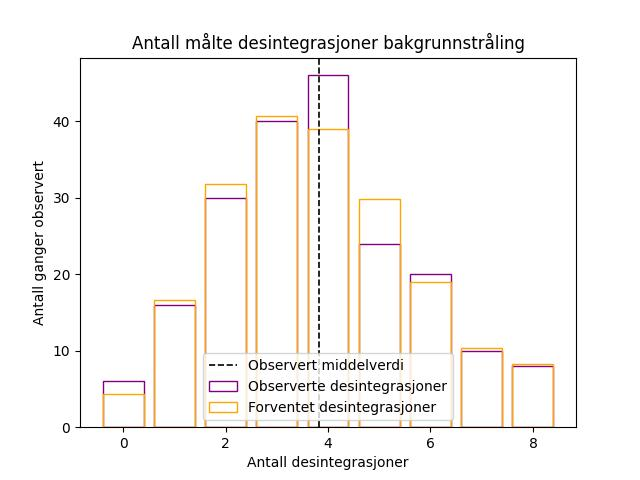
\includegraphics[width=0.5\textwidth]{images/Background_radiation.jpg}
\caption{Bakgrunns desintegrasjon fordelt i ni grupper sammenlignet med Poissonfordeling og middelverdien}
\label{Background_radiation}
\end{figure}


\subsection{Totale strålingen} \label{Totale strålingen}
Middelverdi for total stråling ble beregnet med formel \eqref{Middelverdi formel} og ga en verdi på
\textit{$\bar\nu$} = 1670.84

Standardavvik for total stråling  med  antakelsen om at den underliggende fordelingen er normalfordeling ble beregnet med formel \eqref{Standardavvik} og ga
\textit{$\sigma_\nu$} = 37.55

Standardavvik for total stråling  med  antakelsen om at den underliggende fordelingen er poissonfordeling ble beregnet med formel \eqref{standardavvik poisson}
\textit{$\sigma_{\bar\nu}$} = 40.87

Standard feil for total stråling  med  antakelsen om at den underliggende fordelingen er normalfordeling ble beregnet med formel \eqref{Standardavvik} og ga
\textit{$\sigma_\nu$} = 2.65.

\begin{figure}[ht]
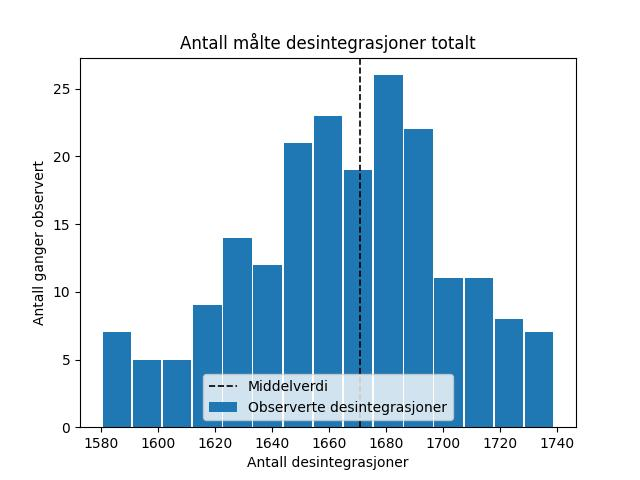
\includegraphics[width=0.5\textwidth]{images/Total_radiation.jpg}
\caption{Desintegrasjon av kilde- og bakgrunnsstråling delt i 15 like store grupper, samt middelverdien.}
\label{Total_radiation}
\end{figure}


\subsection{Strålekilden}
Ut i fra beregninger gjort i \ref{Bakgrunnsstråling} og \ref{Totale strålingen} kan en beregne strålingen fra kun strålekilden. Ved bruk av formel \eqref{Kilde middelverdi} og \eqref{kilde standardavvik} regnes det ut at strålekilden desintegrerer med en rate på 1667.02 $\pm$ 2.65 hvert tiende sekund.
\bigskip

Alle beregningen ble gjort i Python, se vedlegg \ref{Python}.
Rådata er vedlagt og kan sees i vedlegg \ref{RådataVedlegg}.


\section{Diskusjon}

For bakgrunnsstrålingen er det to hypoteser som skal testest. \textit{$H_0 = Poissonfordeling$} og \textit{$H_1 = Normalfordeling$}. Altså at målingene for bakgrunnsstrålingen enten følger poissonfordeling eller normalfordeling. Dette kan testes enkelt ved hjelp av en \textit{$\chi^2$}-test.
Dette ble beregnet tidligere i rapporten for bakgrunnsstrålingen og resultatet fra denne testen sier at bakgrunnstålingen er 81.18$\%$ lik poissonfordelingen. Ettersom dette resultatet er så høyt kan en forkaste \textit{$H_1$} hypotesen og si at \textit{$H_0$} hypotesen står. Dette svaret stemmer også overens i Figur \ref{Background_radiation} hvor en kan se at målingene stemmer ganske overens med de forventete Poissonfordelingen.

Fordi bakgrunnsstrålingen følger poissonfordelingen så kan en si at det elektriske måleinstrumentet, Geiger-Müller-telleren ikke er noe alvorlig feil med. Det kan være systematiske feil, men dette påvirker ikke fordelingen av dataene.

Når en ser på resultatet fra standaravik på bakgrunnsstrålingen med
antakelsen om at den underliggende fordelingen
er normalfordeling, og når den er Poissonfordelingen, kan en se likheter. Det at det er likheter kan tilsi at bakgrunnstrålingen også er normalfordelt.

Fordi bakgrunnsstrålingen hovedsakelig bare består av gammastråling på grunn av alfa- og beta-strålingens begrensede rekkevidde vil ikke eventuelle kilder til alfa- og beta-stråling registreres\cite{radioaktivitet}. Det som kan påvirke målingene er de andre strålekildene som de andre studentene brukte for sine eksperimenter. Når gruppen målte den totale strålingen og bakgrunnsstrålingen så var det ujevnt antall strålekilder i rommet. Noen av disse kan ha utstrålt langdistanse nukleær stråling(gammastråling) som kan ha påvirket målingene og gjort de ujevne.

En annen feilkilde kan være tilfeldige personlige feil. Sånn som å bruke feil formel, notere feil tall eller å skrive koden feil. Det er dokumentert med vedlegg koden som er brukt og rådataene som er henholdsvis vedlegg \ref{Python} og vedlegg \ref{RådataVedlegg}. Dette kan gjøre resultatene helt feil. Data som eventuelt har blitt plottet inn feil vil ikke ha så stor påvirkning på resultatet siden det er så mye data. Ser en i figur \ref{Total_radiation} kan en se tegn til normalfordelingen, dette kan verken avkreftes eller bekreftes uten en kji-kvadrat test.


\section{Konklusjon}
Antall desintegrasjoner i bakgrunnsstrålingen ble målt til 3.83 \textit{$\pm$} 0.15 desintegrasjoner per 10s og følger poissonfordelingen. Dette er 81$\%$ sikkert som følge av \textit{$\chi^2$}-testen som ble gjennomført for å sammenlikne fordelingen med poissonfordelingen. For den totale strålingen er det beregnet 1667.015 \textit{$\pm$} 2.65 desintegrasjoner per 10s antatt normalfordeling. Diagrammet for den totale strålingen kan minne om normalfordelingen, man man kan ikke si noe sikkert uten en kji-kvadrat test.


\bibliographystyle{plain}
\bibliography{sources.bib}
\clearpage

\onecolumn
\newpage
\appendix
\section{Vedlegg A}
\label{Python}

\begin{lstlisting}

    # Imports to make calculation and plotting
    import numpy as np
    import matplotlib.pyplot as plt
    import decimal


    # Function to read data from csv file
    # Input is a csv file of values
    # Returns two list, one for total decay chain and one for background decay chain
    def read_from_csv(file_name):
        list_of_tot = []
        list_of_back = []
        with open(file_name) as file:
            for line in file:
                line = line.split(";")
                line = [k.strip() for k in line]
                list_of_tot.append(int(line[-1]))
                list_of_back.append(int(line[1]))

        return list_of_tot, list_of_back


    # Function to calculate middle value based on list of values
    # Input is a list of numbers used to calculate middle value
    # Returns the middle value as float
    def find_middle_value(list_of_numbers):
        n = len(list_of_numbers)
        number_freq = {}
        answer = 0
        for k, number_func in enumerate(list_of_numbers):
            try:
                number_freq[number_func] += 1
            except KeyError:
                number_freq[number_func] = 1

        for key_func, value_func in number_freq.items():
            answer += key_func * value_func

        return answer / n


    # Function to calculate sigma based on normal distribution
    # Input is a list of observed values and the middle value
    # Returns the standard deviation as float
    def sigma_norm(list_of_nu, my):
        list_to_ans = []
        for k, nu in enumerate(list_of_nu):
            ans = (nu - my) ** 2
            list_to_ans.append(ans)
        sigma = np.sqrt(sum(list_to_ans) / (len(list_of_nu) - 1))

        return sigma


    # Function to calculate sigma based on normal distribution and middle value
    # Input is a list of observed values and the middle value
    # Returns the standard deviation as float
    def sigma_norm_mid(sd, list_of_nu):
        ans = sd / np.sqrt(len(list_of_nu))
        return ans


    # Function to calculate poisson distribution
    # Input is a list of observed values and the middle value
    # Returns the poisson distribution as dictionary, with value as key and number of times
    # that value will accrue as value in percentage
    def poisson(my_1, list_of_nu1):
        decimal.getcontext().prec = 100  # Number of decimal
        ans_dict = {}
        list_of_nu = list(range(min(list_of_nu1), max(list_of_nu1) + 1))
        for k, nu in enumerate(list_of_nu):
            ans = decimal.Decimal(np.e) ** decimal.Decimal(-my_1) * \
                  ((decimal.Decimal(my_1) ** nu) / decimal.Decimal(np.math.factorial(nu)))
            ans_dict[nu] = float(ans)
        return ans_dict


    # Function to calculate sigma based on poisson distribution
    # Input is the middle value
    # Returns the standard deviation as float
    def sigma_poisson(my):
        return np.sqrt(my)


    # Function to calculate chi-square test
    # Input is two list, the observed data and the expected data
    # Returns the chi-square value as float
    def chi_square(observed_data, expected_data):
        list_el = []
        for k in range(len(observed_data)):
            ans = observed_data[k] - expected_data[k]
            ans1 = ans ** 2 / expected_data[k]
            list_el.append(ans1)

        return sum(list_el)


    # Function to calculate only the source decay
    # Input is four values, the middle value and the standard deviation for total decay,
    # the middle value the standard deviation for background decay
    # Returns two float numbers, the middle value and the standard deviation
    def calculate_source_gamma(my_tot, sd_tot, my_back, sd_back):
        my_ans = my_tot - my_back
        sd_ans = np.sqrt(sd_tot ** 2 + sd_back ** 2)
        return my_ans, sd_ans


    # Function to turn list into dictionary
    # Input is a list with keys
    # Returns dictionary of number of times a key occurs
    def list_to_dict(total_list):
        dict_func = {}
        for k, number_funct in enumerate(total_list):  # list_number_tot
            try:
                dict_func[number_funct] += 1
            except KeyError:
                dict_func[number_funct] = 1
        return dict_func


    if __name__ == '__main__':

        # Read csv data into to lists, one for total decay and one for background
        list_number_tot, list_number_back = read_from_csv('data.csv')

        # Middle value for total and background decay
        my1 = find_middle_value(list_number_tot)
        my2 = find_middle_value(list_number_back)

        # Standard deviation for total and background decay based on normal distribution
        sd_norm1 = sigma_norm(list_number_tot, my1)
        sd_norm2 = sigma_norm(list_number_back, my2)

        # Standard error for total and background decay based on normal distribution
        sd_mid1 = sigma_norm_mid(sd_norm1, list_number_tot)
        sd_mid2 = sigma_norm_mid(sd_norm2, list_number_back)

        # Standard deviation for total and background decay based on poisson distribution
        sd_pos1 = sigma_poisson(my1)
        sd_pos2 = sigma_poisson(my2)

        print('-------------------')
        print('Målinger bakgrunnstårling\n')
        print('Middelverdi =', my2, ' Standaravvik normal =', sd_norm2, 'Standarfeil = ', sd_mid2,
              'Standaravvik poisson =', sd_pos2)

        # Turn number of observation to dictionary with frequency of occurrence
        number_freq_observed = list_to_dict(list_number_back)

        # Calculate poisson distribution
        list_of_pos = poisson(my2, number_freq_observed.keys())
        for key in list_of_pos:
            list_of_pos[key] *= 200  # Turn percentage into number of times it will occur with
                                     # 200 readings
        number_freq_expected = list_of_pos

        # Sort dictonary
        myKeys = list(number_freq_observed.keys())
        myKeys.sort()
        number_freq_observed = {i: number_freq_observed[i] for i in myKeys}

        # Sum the last bins to get bin value over 5
        number_freq_observed[8] = number_freq_observed[8] + number_freq_observed[9] + \
            number_freq_observed[11] + number_freq_observed[12]
        del number_freq_observed[9]
        del number_freq_observed[11]
        del number_freq_observed[12]
        number_freq_expected[8] = number_freq_expected[8] + number_freq_expected[9] + \
            number_freq_expected[10] + number_freq_expected[11] + \
            number_freq_expected[12]
        del number_freq_expected[9]
        del number_freq_expected[10]
        del number_freq_expected[11]
        del number_freq_expected[12]

        # Calculate chi-squared
        x_squared = chi_square(list(number_freq_observed.values()), list(number_freq_expected.values()))
        print('x_squared =', x_squared)

        # Define number of degrees of freedom
        df = 7

        # Calculate chi-squared tilde
        x_tilde = x_squared / df
        print('x_tilde', x_tilde)

        # Plot observed background decay with poisson distribution
        width = 1
        plt.bar(number_freq_observed.keys(), number_freq_observed.values(),
                edgecolor='purple', color='None', label='Observerte desintegrasjoner')
        plt.bar(number_freq_expected.keys(), number_freq_expected.values(),
                edgecolor='orange', color='None', label='Forventet desintegrasjoner')
        plt.axvline(my2, color='k', ls='dashed', linewidth=1.2, label='Observert middelverdi')
        plt.xlabel('Antall desintegrasjoner')
        plt.ylabel('Antall ganger observert')
        plt.title('Antall målte desintegrasjoner bakgrunnstråling')
        plt.legend(loc='lower center')
        plt.show()

        print('-------------------')
        print('Målinger med strålekilden\n')
        print('Middelverdi =', my1, 'Standaravvik =', sd_norm1, 'Standaravik poisson =', sd_pos1)

        # Turn number of observation to dictionary with frequency of occurrence
        number_freq_observed1 = list_to_dict(list_number_tot)

        # Divide into bins to get each bin value over 5
        a = sorted(number_freq_observed1)
        bins = np.linspace(min(a), max(a), 20)
        list_with_bins_obs1 = []
        for i, number in enumerate(list(bins)):
            temp_value1 = 0
            for j, value in enumerate(number_freq_observed1.keys()):
                if bins[i] <= value <= bins[i + 1]:
                    temp_value1 += number_freq_observed1[value]
                if i + 1 >= len(list(bins)):
                    break
            list_with_bins_obs1.append(temp_value1)

        # Sum last and first bins to get bin value over 5
        list_with_bins_obs1[-5] = list_with_bins_obs1[-5] + list_with_bins_obs1[-4] + \
            list_with_bins_obs1[-3] + list_with_bins_obs1[-2] + \
            list_with_bins_obs1[-1]
        list_with_bins_obs1[1] = list_with_bins_obs1[1] + list_with_bins_obs1[0]
        list_with_bins_obs1 = list_with_bins_obs1[1:-4]
        bins = bins[1:-4]

        # Plot the total decay
        plt.bar(bins, list_with_bins_obs1, width=10, linewidth=2, label='Observerte desintegrasjoner')
        plt.title('Antall målte desintegrasjoner totalt')
        plt.axvline(my1, color='k', linestyle='dashed', linewidth=1.2, label='Middelverdi')
        plt.xlabel('Antall desintegrasjoner')
        plt.ylabel('Antall ganger observert')
        plt.legend(loc='lower center')
        plt.show()

        print('-------------------')
        print('Måling kun stråling\n')

        # Calculate the decay of only source
        source_my, source_sd = calculate_source_gamma(my1, sd_mid1, my2, sd_mid2)
        print('Middelverdi =', source_my, 'Standarfeil', source_sd)
        print('-------------------')


    \end{lstlisting}

\newpage
\section{Vedlegg B}
\label{RådataVedlegg}
\begin{longtable}{lll}
Måling nummer & Stråling Bakgrunn & Stråling Totalt \\
\endfirsthead
%
\endhead
%
1         & 6        & 1628     \\
2         & 3        & 1655     \\
3         & 3        & 1717     \\
4         & 6        & 1588     \\
5         & 5        & 1664     \\
6         & 2        & 1631     \\
7         & 6        & 1729     \\
8         & 4        & 1705     \\
9         & 3        & 1638     \\
10        & 7        & 1717     \\
11        & 3        & 1678     \\
12        & 3        & 1610     \\
13        & 0        & 1714     \\
14        & 1        & 1692     \\
15        & 4        & 1699     \\
16        & 2        & 1713     \\
17        & 2        & 1637     \\
18        & 9        & 1693     \\
19        & 4        & 1720     \\
20        & 8        & 1687     \\
21        & 9        & 1690     \\
22        & 2        & 1714     \\
23        & 4        & 1743     \\
24        & 3        & 1687     \\
25        & 6        & 1595     \\
26        & 12       & 1700     \\
27        & 5        & 1756     \\
28        & 4        & 1640     \\
29        & 2        & 1693     \\
30        & 7        & 1684     \\
31        & 5        & 1660     \\
32        & 2        & 1700     \\
33        & 2        & 1708     \\
34        & 3        & 1703     \\
35        & 3        & 1685     \\
36        & 4        & 1628     \\
37        & 5        & 1716     \\
38        & 5        & 1627     \\
39        & 4        & 1686     \\
40        & 6        & 1595     \\
41        & 5        & 1635     \\
42        & 4        & 1711     \\
43        & 4        & 1702     \\
44        & 5        & 1688     \\
45        & 7        & 1635     \\
46        & 6        & 1689     \\
47        & 6        & 1750     \\
48        & 1        & 1776     \\
49        & 4        & 1649     \\
50        & 5        & 1708     \\
51        & 3        & 1604     \\
52        & 4        & 1680     \\
53        & 7        & 1630     \\
54        & 0        & 1708     \\
55        & 4        & 1657     \\
56        & 4        & 1687     \\
57        & 3        & 1662     \\
58        & 5        & 1659     \\
59        & 3        & 1652     \\
60        & 3        & 1680     \\
61        & 3        & 1689     \\
62        & 5        & 1677     \\
63        & 2        & 1691     \\
64        & 4        & 1648     \\
65        & 1        & 1697     \\
66        & 5        & 1663     \\
67        & 1        & 1662     \\
68        & 3        & 1679     \\
69        & 4        & 1677     \\
70        & 3        & 1641     \\
71        & 2        & 1658     \\
72        & 6        & 1671     \\
73        & 1        & 1687     \\
74        & 4        & 1681     \\
75        & 2        & 1695     \\
76        & 1        & 1679     \\
77        & 9        & 1688     \\
78        & 4        & 1697     \\
79        & 4        & 1656     \\
80        & 4        & 1737     \\
81        & 4        & 1651     \\
82        & 1        & 1645     \\
83        & 3        & 1673     \\
84        & 3        & 1652     \\
85        & 2        & 1728     \\
86        & 5        & 1656     \\
87        & 2        & 1663     \\
88        & 3        & 1663     \\
89        & 3        & 1670     \\
90        & 0        & 1632     \\
91        & 6        & 1618     \\
92        & 1        & 1663     \\
93        & 3        & 1733     \\
94        & 1        & 1693     \\
95        & 3        & 1618     \\
96        & 4        & 1622     \\
97        & 6        & 1653     \\
98        & 2        & 1702     \\
99        & 3        & 1731     \\
100       & 9        & 1696     \\
101       & 4        & 1637     \\
102       & 3        & 1594     \\
103       & 6        & 1658     \\
104       & 3        & 1589     \\
105       & 6        & 1722     \\
106       & 2        & 1653     \\
107       & 1        & 1671     \\
108       & 6        & 1694     \\
109       & 2        & 1648     \\
110       & 4        & 1646     \\
111       & 6        & 1635     \\
112       & 6        & 1670     \\
113       & 4        & 1738     \\
114       & 1        & 1679     \\
115       & 1        & 1602     \\
116       & 6        & 1666     \\
117       & 4        & 1655     \\
118       & 7        & 1654     \\
119       & 2        & 1617     \\
120       & 3        & 1668     \\
121       & 5        & 1724     \\
122       & 1        & 1620     \\
123       & 0        & 1665     \\
124       & 3        & 1727     \\
125       & 4        & 1686     \\
126       & 7        & 1700     \\
127       & 5        & 1661     \\
128       & 4        & 1667     \\
129       & 4        & 1667     \\
130       & 3        & 1650     \\
131       & 3        & 1675     \\
132       & 9        & 1689     \\
133       & 3        & 1661     \\
134       & 4        & 1680     \\
135       & 5        & 1671     \\
136       & 5        & 1656     \\
137       & 11       & 1675     \\
138       & 4        & 1632     \\
139       & 5        & 1630     \\
140       & 2        & 1642     \\
141       & 3        & 1690     \\
142       & 3        & 1674     \\
143       & 3        & 1662     \\
144       & 5        & 1671     \\
145       & 2        & 1641     \\
146       & 2        & 1702     \\
147       & 4        & 1652     \\
148       & 7        & 1620     \\
149       & 4        & 1647     \\
150       & 0        & 1763     \\
151       & 4        & 1610     \\
152       & 4        & 1669     \\
153       & 4        & 1694     \\
154       & 7        & 1688     \\
155       & 3        & 1681     \\
156       & 4        & 1689     \\
157       & 4        & 1700     \\
158       & 2        & 1704     \\
159       & 1        & 1598     \\
160       & 2        & 1700     \\
161       & 3        & 1706     \\
162       & 4        & 1651     \\
163       & 3        & 1624     \\
164       & 5        & 1607     \\
165       & 3        & 1691     \\
166       & 5        & 1657     \\
167       & 2        & 1679     \\
168       & 2        & 1603     \\
169       & 4        & 1717     \\
170       & 3        & 1682     \\
171       & 4        & 1654     \\
172       & 2        & 1688     \\
173       & 2        & 1575     \\
174       & 2        & 1729     \\
175       & 4        & 1624     \\
176       & 5        & 1631     \\
177       & 4        & 1619     \\
178       & 3        & 1603     \\
179       & 0        & 1639     \\
180       & 2        & 1662     \\
181       & 6        & 1667     \\
182       & 5        & 1645     \\
183       & 2        & 1687     \\
184       & 7        & 1687     \\
185       & 6        & 1693     \\
186       & 7        & 1617     \\
187       & 2        & 1677     \\
188       & 5        & 1730     \\
189       & 2        & 1690     \\
190       & 4        & 1699     \\
191       & 4        & 1693     \\
192       & 3        & 1716     \\
193       & 6        & 1667     \\
194       & 1        & 1693     \\
195       & 5        & 1722     \\
196       & 6        & 1580     \\
197       & 3        & 1665     \\
198       & 4        & 1696     \\
199       & 1        & 1654     \\
200       & 4        & 1699
\end{longtable}
\end{document}

